\newpage
\solutions{Konstrukcje}

\begin{problem}{1} 
	Wykazać, że można pokolorować $40$ pól na nieskończonej szachownicy, tak, aby nie istniał prostokąt utworzony z pól tej szachownicy zawierający dokładnie $20$ pokolorowanych pól.
\end{problem}

\noindent
Rozpatrzmy kolorowanie takie jak na rysunku - pola, w które wpisano literę są pomalowane.

\begin{center}
    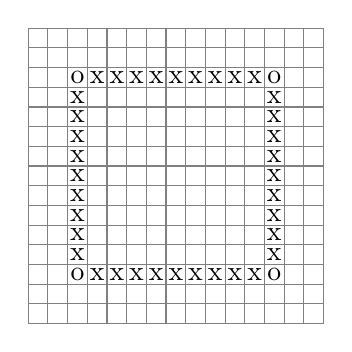
\begin{tikzpicture}[x=1cm, scale=0.25]
    \foreach \y in {-1,0,...,12}{
        \foreach \x in {-1,0,...,12}{
            \draw[black!50] (\x,\y) rectangle (1+\x,1+\y) rectangle (2+\x,2+\y);}}

    \draw[black!50] (-1,-1)--(14,-1)--(14,14)--(-1,14)--cycle;
    \node at (1.5,1.5) {o};
    \node at (2.5,1.5) {x};
    \node at (3.5,1.5) {x};
    \node at (4.5,1.5) {x};
    \node at (5.5,1.5) {x};
    \node at (6.5,1.5) {x};
    \node at (7.5,1.5) {x};
    \node at (8.5,1.5) {x};
    \node at (9.5,1.5) {x};
    \node at (10.5,1.5) {x};
    \node at (11.5,1.5) {o};

    \node at (1.5,11.5) {o};
    \node at (2.5,11.5) {x};
    \node at (3.5,11.5) {x};
    \node at (4.5,11.5) {x};
    \node at (5.5,11.5) {x};
    \node at (6.5,11.5) {x};
    \node at (7.5,11.5) {x};
    \node at (8.5,11.5) {x};
    \node at (9.5,11.5) {x};
    \node at (10.5,11.5) {x};
    \node at (11.5,11.5) {o};

    \node at (11.5,2.5) {x};
    \node at (11.5,3.5) {x};
    \node at (11.5,4.5) {x};
    \node at (11.5,5.5) {x};
    \node at (11.5,6.5) {x};
    \node at (11.5,7.5) {x};
    \node at (11.5,8.5) {x};
    \node at (11.5,9.5) {x};
    \node at (11.5,10.5) {x};

    \node at (1.5,2.5) {x};
    \node at (1.5,3.5) {x};
    \node at (1.5,4.5) {x};
    \node at (1.5,5.5) {x};
    \node at (1.5,6.5) {x};
    \node at (1.5,7.5) {x};
    \node at (1.5,8.5) {x};
    \node at (1.5,9.5) {x};
    \node at (1.5,10.5) {x};

    \end{tikzpicture}
\end{center}

\noindent
Zauważmy, że jeśli pewien prostokąt nie przykrywa żadnego pola z literą o, to może zawierać co najwyżej $18$ pokolorowanych pól. Jeśli zawiera tylko jedną, to może zawierać ich co najwyżej $19$. Jeśli zaś zawiera on w całości pewną ,,krawędź'' pokolorowanego prostokąta, to albo zawiera nieparzystą liczbę pól, albo zawiera je wszystkie. Więc szukany prostokąt nie istnieje.

\vspace{10px}

\begin{problem}{2} 
	Udowodnij, że punkty płaszczyzny można tak pokolorować dziewięcioma kolorami, aby żadne dwa punkty odległe o 1 nie były tego samego koloru.
\end{problem}

\noindent
Podzielmy płaszczyznę na kratkę, tak że przekątna każdej kratki ma długość $1$. Kolorujemy wszystkie punkty wewnątrz kratki, jej dolną krawędź bez prawego wierzchołka i jej lewą krawędź bez górnego wierzchołka na kolor przypisany według sposobu zademonstrowanego na lewym rysunku. 

\begin{center}
    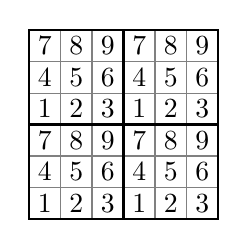
\begin{tikzpicture}[x=1cm, scale=0.4]
    \foreach \y in {0,...,4}{
        \foreach \x in {0,...,4}{
            \draw[black!50] (\x,\y) rectangle (1+\x,1+\y) rectangle (2+\x,2+\y);}}

    \draw[black!50] (0,0)--(6,0)--(6,6)--(0,6)--cycle;
    \draw[line width=1] (0,0)--(3,0)--(3,3)--(0,3)--cycle;
    \draw[line width=1] (0,3)--(3,3)--(3,6)--(0,6)--cycle;
    \draw[line width=1] (3,0)--(6,0)--(6,3)--(3,3)--cycle;
    \draw[line width=1] (3,3)--(6,3)--(6,6)--(3,6)--cycle;
    \node at (0.5,0.5) {1};
    \node at (1.5,0.5) {2};
    \node at (2.5,0.5) {3};
    \node at (3.5,0.5) {1};
    \node at (4.5,0.5) {2};
    \node at (5.5,0.5) {3};


    \node at (0.5,1.5) {4};
    \node at (1.5,1.5) {5};
    \node at (2.5,1.5) {6};
    \node at (3.5,1.5) {4};
    \node at (4.5,1.5) {5};
    \node at (5.5,1.5) {6};



    \node at (0.5,2.5) {7};
    \node at (1.5,2.5) {8};
    \node at (2.5,2.5) {9};
    \node at (3.5,2.5) {7};
    \node at (4.5,2.5) {8};
    \node at (5.5,2.5) {9};

    \node at (0.5,3.5) {1};
    \node at (1.5,3.5) {2};
    \node at (2.5,3.5) {3};
    \node at (3.5,3.5) {1};
    \node at (4.5,3.5) {2};
    \node at (5.5,3.5) {3};


    \node at (0.5,4.5) {4};
    \node at (1.5,4.5) {5};
    \node at (2.5,4.5) {6};
    \node at (3.5,4.5) {4};
    \node at (4.5,4.5) {5};
    \node at (5.5,4.5) {6};



    \node at (0.5,5.5) {7};
    \node at (1.5,5.5) {8};
    \node at (2.5,5.5) {9};
    \node at (3.5,5.5) {7};
    \node at (4.5,5.5) {8};
    \node at (5.5,5.5) {9};

    \end{tikzpicture}
    \hspace{30px}
    \begin{tikzpicture}[x=1cm, scale=0.4]
    \draw[line width=1] (0,0)--(4,0);
    \draw[line width=1] (0,0)--(0,4);
    \node at (0,0)[circle,fill,inner sep=1.5pt]{};
    %\node at (0,4)[circle,fill=white,draw,outer sep=0pt,inner sep=1.5pt]{};
    %\node at (4,0)[circle,fill=white,draw,outer sep=0pt,inner sep=1.5pt]{};
    \fill[pattern=north west lines] (0,0) rectangle (4,4);
    \end{tikzpicture}
\end{center}

\noindent
Łatwo zauważyć, że takie kolorowanie spełnia warunki zadania.

\begin{problem}{3}
	Wykazać, że każdy trójkąt można podzielić na $3000$ czworokątów wypukłych, tak, aby każdy z nich dało się wpisać w okrąg oraz opisać na okręgu.
\end{problem}

\noindent
Na początku wykażemy, że każdy trójkąt można podzielić na $3$ takie czworokąty. Rozpatrzmy dowolny trójkąt $ABC$. Niech $I$ to będzie środek okręgu weń wpisanego, a punkty $D$, $E$ i $F$ to będą rzuty $I$ odpowiednio na boki $BC$, $CA$ i $AB$. Zauważmy, że $IE = IF$(promienie okręgu) oraz $AF = AE$(odcinki styczne). Stąd $AF + IE = AE + IF$, czyli czworokąt $AFIE$ da się opisać na okręgu. Mamy też, że kąty $\an AFI$ i $\an AEI$ są proste, czyli czworokąt $AFIE$ da się wpisać w okrąg. Analogicznie rozumujemy dla czworokątów $BDIF$ oraz $CEID$.

\begin{center}
	\begin{tikzpicture}
		\tkzDefPoint(0,0){A}
		\tkzDefPoint(5,0){B}
		\tkzDefPoint(3,2){C}

		\tkzDefTriangleCenter[in](A,B,C)\tkzGetPoint{I}
		\tkzDefPointsBy[projection=onto B--C](I){D}
		\tkzDefPointsBy[projection=onto C--A](I){E}
		\tkzDefPointsBy[projection=onto A--B](I){F}


		\tkzDrawPoints(A,B,C, I, D,E,F)
		\tkzDrawSegments(A,B B,C C,A I,D I,E I,F)
		\tkzDrawCircle[dashed](I,F)
		\tkzLabelPoints[below](A,B, F)
		\tkzLabelPoints[above](C)
		\tkzLabelPoints[left](I)
		\tkzLabelPoints[above left](E)
		\tkzLabelPoints[above right](D)
		\tkzMarkRightAngle[german](I,F,A)
		\tkzMarkRightAngle[german](A,E,I)
	\end{tikzpicture}
	\hspace{10px}
	\begin{tikzpicture}
		\tkzDefPoint(0,0){A}
		\tkzDefPoint(5,0){B}
		\tkzDefPoint(3,2){C}
		\tkzDefPoint(1,0){X_1}
		\tkzDefPoint(2,0){X_2}
		\tkzDefPoint(4,0){X_{999}}
		\tkzDefPoint(3,0){T}

		\tkzDefTriangleCenter[in](A,B,C)\tkzGetPoint{I}
		\tkzDefPointsBy[projection=onto B--C](I){D}
		\tkzDefPointsBy[projection=onto C--A](I){E}
		\tkzDefPointsBy[projection=onto A--B](I){F}


		\tkzDrawPoints(A,B,C, X_1, X_2, X_{999})
		\tkzDrawSegments(C,X_1 C,X_2 C,X_{999})
		\tkzDrawSegments(A,B B,C C,A)
		\tkzLabelPoints[below](A,B,X_1, X_2, X_{999})
		\tkzLabelPoints[above](C)
		\tkzLabelPoint[below](T){$\dots$}
	\end{tikzpicture}
\end{center}

\noindent
Wystarczy więc podzielić wyjściowy trójkąt na $1000$ trójkątów jak na rysunku $1$, a następnie każdy z tych trójkątów podzielić na $3$ szukane czworokąty.

\vspace{10px}

\begin{problem}{4} 
	Wykazać, że można pokolorować każdą dodatnią liczbę całkowitą na jeden z $1000$ kolorów, tak aby
	\begin{itemize}
		\item każdy z kolorów był użyty nieskończenie wiele razy;
		\item dla dowolnych takich liczb całkowitych $a$, $b$, $c$, że $ab = c$, pewne dwie spośród nich sa jednakowego koloru.
	\end{itemize} 
\end{problem}

\vspace{5px}

\noindent
Przyjmijmy $p_1 = 2,\; p_2 = 3, \; ...$ jako kolejne liczby pierwsze. Liczbę $1$ kolorujemy dowolnym kolorem. Niech $p_i$ to będzie najmniejszy dzielnik pierwszy pewnej liczby $n$. Wówczas jeśli $i \leqslant 1000$ kolorujemy $n$ kolorem o numerze $i$. W przeciwnym wypadku kolorujemy go kolorem o numerze $1000$.

\vspace{5px}

\noindent
Wykażemy, że podane kolorowanie spełnia warunki zadania. Łatwo zauważyć, że każdy z kolorów będzie użyty nieskończenie wiele razy. Załóżmy więc, że $ab = c$. Jeśli jedna z liczb $a$, $b$ jest równa jeden, to pozostałe są równe, więc w szczególności są tego samego koloru. Niech $p$ będzie najmniejszym dzielnikiem liczby $abc$. Wówczas, skoro $ab = c$ liczba~$p$ musi dzielić co najmniej dwie spośród $a$, $b$, $c$. Z minimalności $p$ mamy, że wyznaczy ona jednakowy kolor obu tym liczbom.

\vspace{10px}

\begin{problem}{5}
	Łódka może zabrać w rejs po jeziorze dokładnie 7 osób. Udowodnij. że można tak zaplanować rejsy 49-osobowej wycieczki, aby każdych dwóch uczestników płynęło ze sobą dokładnie raz.
\end{problem}

\noindent
Zinterpretujmy te $49$ osób jako planszę 7 na 7, gdzie każdemu polu przyporządkowana jest jedna osoba. Rozpatrzmy wszystkie kolorowania powstające w następujący sposób. Kolorujemy dowolna pola w najniższym i drugim najniższym wierszu. Załóżmy, że są to pola $a$-te i $a + k$-te(być może $k < 0$). Wówczas w trzeciej kolumnie pokolorujemy pole $a + 2k \pmod{7}$, w czwartej $a + 3k \pmod{7}$ itd. Przykładowe kolorowanie dla $a = 2$ i~$k = 2$ jest na rysunku.


\begin{center}
    \begin{tikzpicture}[x=1cm, scale=0.4]
    \foreach \y in {0,...,5}{
        \foreach \x in {0,...,5}{
            \draw[black!50] (\x,\y) rectangle (1+\x,1+\y) rectangle (2+\x,2+\y);}}

    \draw[black!50] (0,0)--(7,0)--(7,7)--(0,7)--cycle;
    
    \fill[pattern=north west lines] (1,0) rectangle (2,1);
    \fill[pattern=north west lines] (3,1) rectangle (4,2);
    \fill[pattern=north west lines] (5,2) rectangle (6,3);
    \fill[pattern=north west lines] (0,3) rectangle (1,4);
    \fill[pattern=north west lines] (2,4) rectangle (3,5);
    \fill[pattern=north west lines] (4,5) rectangle (5,6);
    \fill[pattern=north west lines] (6,6) rectangle (7,7);

    \end{tikzpicture}
\end{center}

\noindent
Rozpatrzmy wszystkie takie kolorowania i dla każdego weźmy osoby przyporządkowane pokolorowanym polom na rejs. Wykażemy, że dowolne dwa pola są jednocześnie pokolorowane w dokładnie jednym kolorowaniu. Przyjmijmy, że te dwa pola są oddalone o $y \neq 0$ wierszy w pionie i $x$ kolumn w poziomie. Zauważmy, że wówczas musi zajść ${x \equiv yk \pmod{7}}$, co jest prawdą dla dokładnie jednego $k$. Skoro $k$ jest jednoznacznie wyznaczone i znamy położenie jednego pola z kolorowania, to możemy odtworzyć położenie wszystkich. Skoro z dwóch pól możemy jednoznacznie odtworzyć kolorowanie, do którego oba należą, to teza jest prawdziwa.


\vspace{10px}
\noindent
Dla każdego kolorowania weźmy osoby odpowiadające pomalowanym polom na rejs. Wówczas każde dwie osoby będą razem na rejsie dokładnie raz, co było do wykazania.

\vspace{10px}

\begin{problem}{6}
	Jaś zapisał pewną skończoną liczbę liczb rzeczywistych na tablicy. Następnie zaczął wykonywać ruchy. W każdym ruchu wybiera dwie równe liczby $a$, $a$, zmazuje je i zapisuje liczby $a + 100$, $a + 2000$. Wykazać, że Jaś może zapisać na początku takie liczby, że będzie mógł wykonywać ruchy w nieskończoność.
\end{problem}

\noindent
Załóżmy, że dla pewnej liczb całkowitych $a$ zapisano liczby
\[
	a,\; a + 1,\; a + 2,\; ...,\; a + 1999 \quad \text{oraz} \quad
	a,\; a + 1,\; a + 2,\; ..., \; a + 99.
\]
Zauważmy, że wykonując ruch zamieniający dwie liczby $a$ na liczby $a + 100$ i $a + 2000$, otrzymujemy analogiczną konfigurację dla $a + 1$. Wypisując na starcie taką konfigurację chociażby dla $a = 0$, Jaś będzie w stanie wykonywać ruchy w nieskończoność.



